\documentclass[a4paper]{article}
\usepackage{fancyhdr}
\usepackage[pdftex]{graphicx}
\usepackage{sidecap}
\usepackage{listings}
\usepackage{color}
\usepackage[export]{adjustbox}
\usepackage{subcaption}

\usepackage{hyperref}
\hypersetup{
    colorlinks=true,
    linkcolor=blue,
    filecolor=magenta, 
    urlcolor=cyan,
    bookmarks=true,
    pdfpagemode=FullScreen,
}
\usepackage{geometry}
 \geometry{
 a4paper,
 total={210mm,297mm},
 left=15mm,
 right=15mm,
 top=15mm,
 bottom=15mm,
 }

\usepackage{glossaries}


\makeglossaries
\newglossaryentry{FSM}
{
    name=FSM,
    description={Finite State Machine}
}

\definecolor{mygreen}{RGB}{25,172,0} % color values Red, Green, Blue
\definecolor{mylilas}{RGB}{170,55,241}
\definecolor{dkgreen}{rgb}{0,0.6,0}
\definecolor{gray}{rgb}{0.5,0.5,0.5}
\definecolor{mauve}{rgb}{0.58,0,0.82}

\pagestyle{fancy}
\fancyhf{}
\rhead{Vangjush Komini}
\lhead{KU Leuven}
\rfoot{Page \thepage}
\lfoot{Biomedical Data Processing part 2}


\lstset{inputpath=Code3}
\graphicspath{{Images3/}}

\include{Glossary}


\begin{titlepage}

\title{Assignment3\\\centerline{\textit{ Blind Source Separation}} }

\author{
\href{mailto:vangjush.komini@uzleuven.be}{Vangjush Komini}\\  \textit{r0612470} \\
\href{mailto:vangjush.komini@uzleuven.be}{vangjush.komini@uzleuven.be}\\
}





\end{titlepage}




\begin{document}



\maketitle
\begin{center}
\Large \href{https://onderwijsaanbod.kuleuven.be/syllabi/e/H06W1AE.htm#activetab=doelstellingen_idp41200}{Biomedical Data Processing, Part II Course}
\end{center}

\begin{figure}[!htbp]
\centering

\includegraphics[width=0.4\textwidth]{icon1.png}
\end{figure}



\section{Q1}
Decomposition of the covariance and the fourth cumulative tensor


After estimating the rank of both of the tensors they appear to both have be rank 2. 

The rank-1 terms for the covariance matrix are in table \ref{a5} and \ref{a6} whereas the rank-1 temrs for the cumulant tensor C4 are in the table \ref{a7} and \ref{a8}.
These component are decomposed via canonical polydiac decomposition CPD where$\#$ is the Khatri-Rao product:

\begin{equation}
C2=\sum_{i=1}^{R}U1_{i}^{(1)}\#U2_{i}^{(2)}
\end{equation}

\begin{equation}
C4=\sum_{i=1}^{R}U11_{i}^{(1)}\#U22_{i}^{(2)}
\end{equation}

The outcome term product $U11_{i}^{(1)}\#U22_{i}^{(2)}$ is of rank 1 tensor.
Moreover $\lambda_{i}$ and $\Lambda_{i}$ are the singular values from the scaling matrix. Generally speaking CPD or any kind of decomposition consist of mainly three matrices.

\begin{equation}
X=ADB^T=\sum_{r}^{R}\lambda_{r}a_{r}b_{r}
\end{equation}
where D is the scaling tensor meaning that its diagonal consist of the scaling singular values. whereas A is the the mixing matrix and last B represent the unknown sources to be estimated\cite{19}. In this case the estimated rank scaling component $\lambda_{i}$ and $\Lambda_{i}$ correspond to its respective diagonal of the D matrix. 

\section{Q2}

Hereby different the sources are additive white gaussian noise at different level. Starting from 5 up to 40 dB with a step of 5dB. In the ICA case the Signal to Interference SIR tends to decay as the level of the noise increases figure \ref{a1} and \ref{a2}. This indicates that the separation tends to be less efficient at higher noise level. Likewise the same happen when the source separation is performed via PCA figure \ref{a3} and \ref{a4}. Although both methods as expected tends to separate less efficiently as the noise level increases. In addition comparing ICA to PCA, the results from the ICA however have a better performance in both cases. Furthermore ICA tries to makes the signals as independent as possible whereas PCA tries to makes the signals as independent as possible. In the case of the ICA independence is much stronger separation consequently the interference tries to be inferior in the ICA scenario. Moreover the 2-norm condition number for the first and the second matrix is fairly higher than on means both mixing matrices are just a bit far from the singularity. This is just the computation ration between the biggest and the smallest singular value. A singular values is somehow undesirable because the interference between the signals will be much higher compare to the the singular case and therefore the SIR tends to be lower. Thi is confirmed even in the processing data from the figures \ref{a1} and \ref{a2}.  


\section{Q3}

Application of the ICA on the FECG data tends to decrease the interference coming from other sources at the region the electrodes of the interest. However in this "cocktail" effect the outcome is not with benefits in all the cases. Hereby in figure \ref{a9} and \ref{a10} the signals before applying ICA tends to contain a lot of interference however in addition a lot of small amplitude signal is also incorporated into the underlying signal. This peaks could potentially disappear after the ICA since their correlation to the noise is much higher compare to the correlation to the real high amplitude signal consequently after ICA these peaks mainly disappear.  Nevertheless these weak fetal signal could potentially be important information for the analysis. The first two channels in the figure \ref{a9} correspond to the last two channel in the figure \ref{a10} respectively. Hereby the amplitudes of each peaks tends to be higher moreover withing peaks more information is retrieved compare to the case before the ICA. Apart from this drawback important information are retrieved at channel 3 and 4 in te figure \ref{a9} indicates much amplitude averagely speaking. This could be due to the high Independence that signals try to achieve and therefore in this case the interference are aimed to be suppressed considerably. 

It is important to reconfirm that the ordering of the channels from ICA is not ensured in addition the polarity of the signals is also random event.

\section{Q4}

The tensor is decomposed into 3 dydiac of rank-1 term. These are plotted into the figure \ref{a15} and it is notable a symmetry for each column and the rank for respective matrix is one. Components are theoretically orthogonal to each other. Therefore these component could be extracted the  T(:,:,4) via PCA. Since PCA still tries to extract two the first two compopnent as as [U S V]=svd(T(:,:,4)). U is this case correspond to the mixing matrix B, V correspond to the source matrix C where S contains the singular values just as in the A matrix. This is an approximate estimaten of this component via SVD. This results are ploted in \ref{A1}

First the multi-linear singular values decomposition is computed for both noiseless and noisy signal. In the noiseless signals the singular values in the figure \ref{a11} tends to decay meaning that the noisy is fairly inferior compare to the the truth signal. Upon superimposing the noisy these low values will be shifted up indicating that higher variance is induced into the signal and some information is therefore shifted into other singular values. 

Regarding the CPD different rank perform different estimation at different iteration length. The algorithm used in this case is nonlinear least squares NLS wherein multiple initialization are used therefore any local optima is avoided in this case. In order to reach the best estimation possible the the stop criteria is put at the order of -20. This will enable a very slow error to be toleration. Further more pseudo-random initialization are used in order explore are more heterogeneous space as possible. CPD performs fairly good at rank close to 11 where from the figure \ref{a13} meaning that high number of iteration is needed to reach the stopping criteria at CPD with rank 12,13,14. Further more the norm in this cases tends to be higher. However throughout all the number of rank tested the relative error tends to be the same since they reach at the same stopping criteria. 



\section{Q5}

Herein the EEG data channels are plotted over different channels in figure \ref{a17}. In order to decompose this signals via CPD tensorization takes place meaning that first mode correspond to time, second mode correspond to frequency and the second mode correspond to the number of channel. This third order tensor is then plotted in figure \ref{a16}. Further more CPD is performed upon this tensor and the outcome will there rank 1 terms. The rank of this tensor is not known therefore after same iteration  of testing posses some interesting properties. Plots in figure \ref{a18} and figure \ref{a19} that in both frequency and time resolution three of the lines are practically identical. In time resolution there is an almost overlap between the red green and the blue line in figure \ref{a18} likewise in the frequency resolution figure \ref{a19} the red green and the dark blue line are nearly symmetric to the x axis. Therefore the minimum terms for rank 1 tensors are three. In addition this two terms are in theory independent from each other due to the to orthogonality of the of component outcomed from the CPD. Since there are different channels targeting independent event from the brain, the goal of the decomposition is acquiring voltage profile at each of the electrodes from these respective events. In the figure \ref{a20} is the voltage profile of the first rank 1 tensor corresponding to the first independent event occurring in the brain. In other words this is were the normal brain activity event occurs located mainly around the forehead of the patient. This is also related to the time resolution figure at the middle plot likewise to the frequency resolution the middle plot is the corresponding component. This is due to the fact that normal brain activities are not associated with high frequency event and potentially any high frequency is an abnormality. 

In the figure \ref{a21} is the second event and at the \ref{a22} and \ref{a23} is the same event plotted at different gray scale. These three plots are logically connected to the remaining of the lines in both time and frequency resolution plots. Practically this is a blind source separation of different events coming from the brain. This voltage map correspond mainly to the epileptic seizure from brain. In case of the seizure and the time resolution of this case is quite high high compare to the normal brain activity and the same will actually happen in frequency resolution where the high frequency events coming from the wavelet are mainly associated to the abnormal. The source is coming from the  indicated part of the brain in figure \ref{a22} as a very strong signal. 

In order to confirm the rank estimation of this tensor in figure \ref{A2} is plotted the norm versus iteration solution using again nonlinear least square. In this figure it is obvious that the convergence of the algorithm is prevalent only for rank equal to two. Higher rank tends to diverge as the numnber of iteration increases.











\newpage


\begin{table}[!htbp]
\centering
\caption{\textbf{\textit{U1:}}Fist component for the covariance matrix}\label{a5}
\begin{tabular}{c c c c c c c c c c c c c c c c c} 
  \hline  
   $-0.4180$&$-0.3272$\\
   $-0.4687$&$0.2652$\\
   $-0.4073$&$0.2599$\\
 \hline
\end{tabular}
\end{table}

  \begin{table}[!htbp]
\centering
\caption{\textbf{\textit{U2:}}Fist component for the covariance matrix}\label{a6}
\begin{tabular}{c c c c c c c c c c c c c c c c c} 
  \hline  

   $-0.7796$&$-0.1053$\\
   $-0.9256$&$ 0.1512$\\
   $-0.8068$&$ 0.1439$\\
 \hline
\end{tabular}
\end{table}


  \begin{table}[!htbp]
\centering
\caption{\textbf{\textit{U11:}}Fist component for the fourth order cumulant tensor}\label{a7}
\begin{tabular}{c c c c c c c c c c c c c c c c c} 
  \hline  
  \hline  
   $-4.6738$&$30.6776$\\
   $-7.4190$&$ 8.0774$\\
   $-6.5489$&$ 5.7962$\\
 \hline
 \hline  
   $-0.5330$&$-0.9670$\\
   $-0.8461$&$-0.2546$\\
   $-0.7469$&$-0.1827$\\
 \hline
 \hline
\end{tabular}
\end{table}

     
  \begin{table}[!htbp]
\centering
\caption{\textbf{\textit{U22:}}Fist component for the fourth order cumulant tensor}\label{a8}
\begin{tabular}{c c c c c c c c c c c c c c c c c} 
  \hline  
  \hline  
   $-0.0691$&$-0.0124$\\
   $-0.1097$&$-0.0033$\\
   $-0.0968$&$-0.0023$\\
 \hline
 \hline  
   $-0.5330$&$ 0.9670$\\
   $-0.8461$&$ 0.2546$\\
   $-0.7469$&$ 0.1827$\\
 \hline
   
 \hline
\end{tabular}
\end{table}

\begin{figure}[!htbp]
\minipage{.47\textwidth}%
\centering
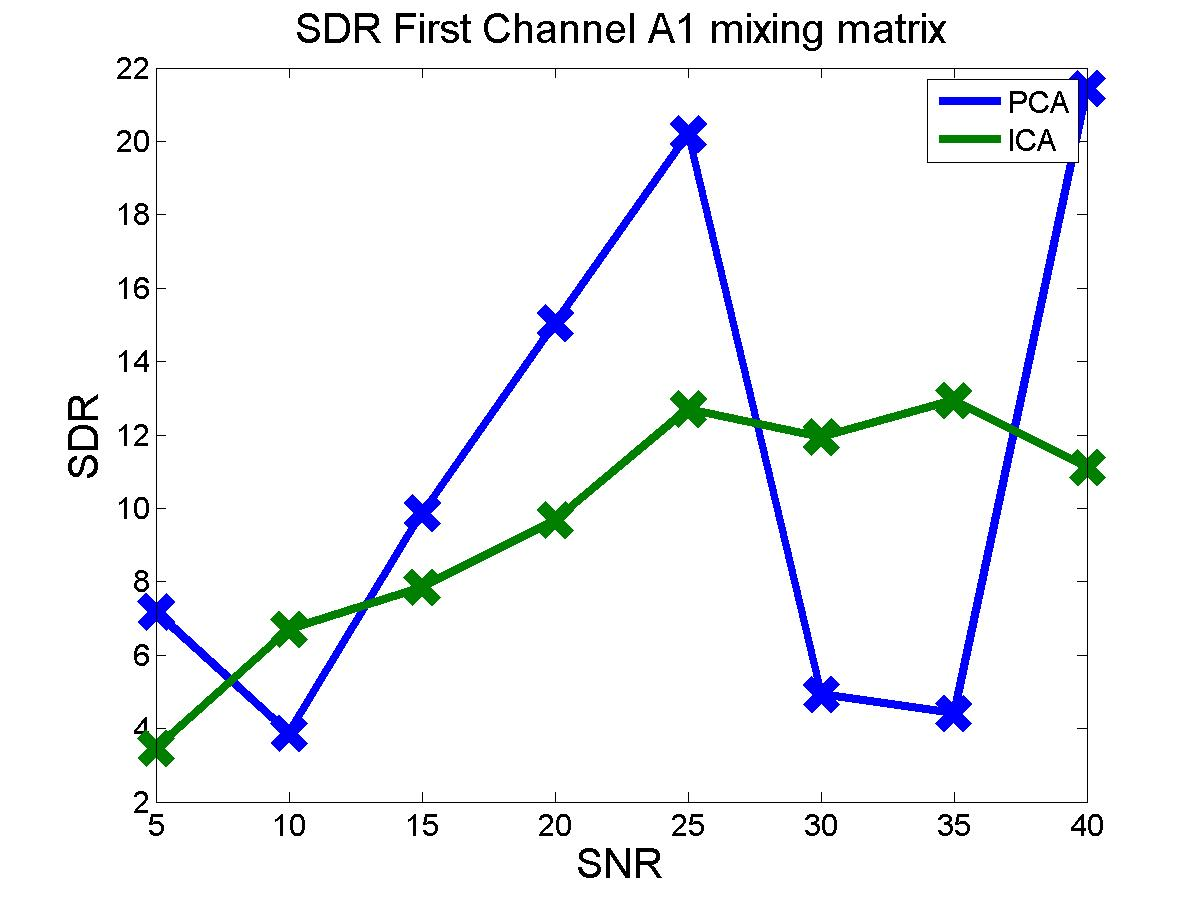
\includegraphics[width=.6\textwidth]{1.jpg}\\
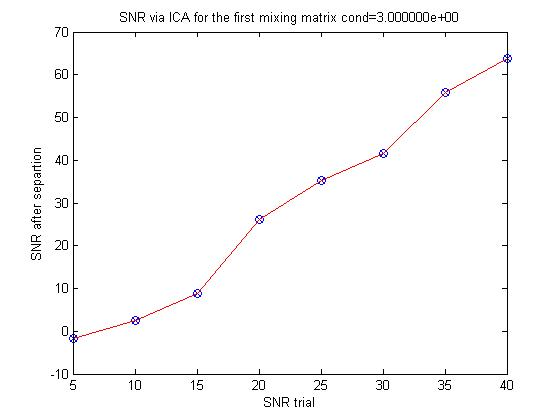
\includegraphics[width=.6\textwidth]{SNR1.jpg}\\
\tiny{First mixing matrix}\label{a1}
\endminipage\hfill
\minipage{.47\textwidth}%
\centering
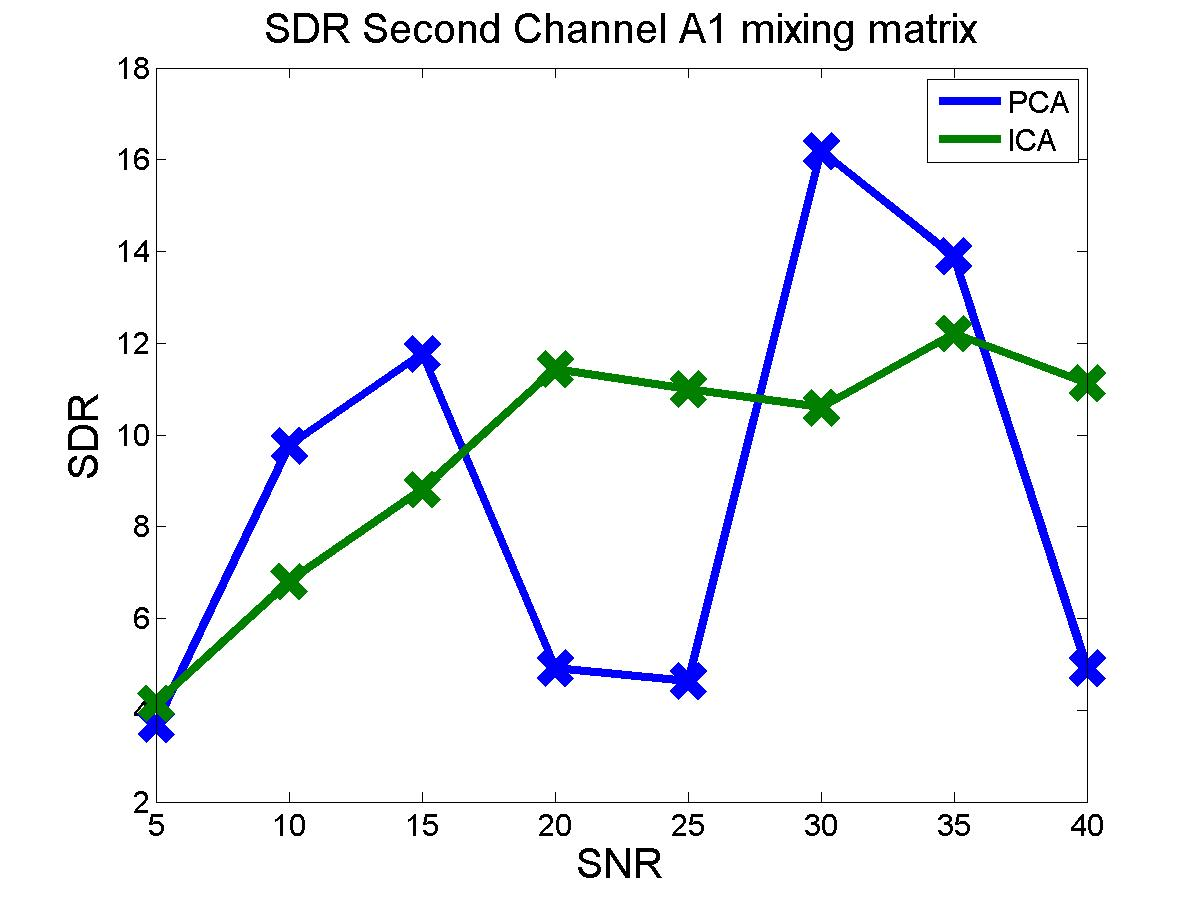
\includegraphics[width=.6\textwidth]{2.jpg}\\
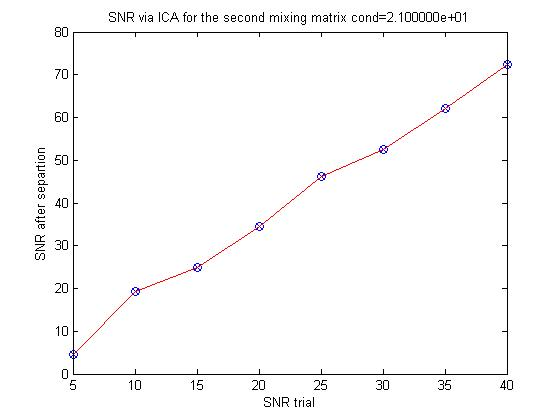
\includegraphics[width=.6\textwidth]{SNR2.jpg}\\
\tiny{Second mixing matrix}\label{a2}
\endminipage\hfill
\caption{\tiny Performance of ICA Implementation}\label{a1}
\end{figure}



\begin{figure}[!htbp]
\minipage{.47\textwidth}%
\centering
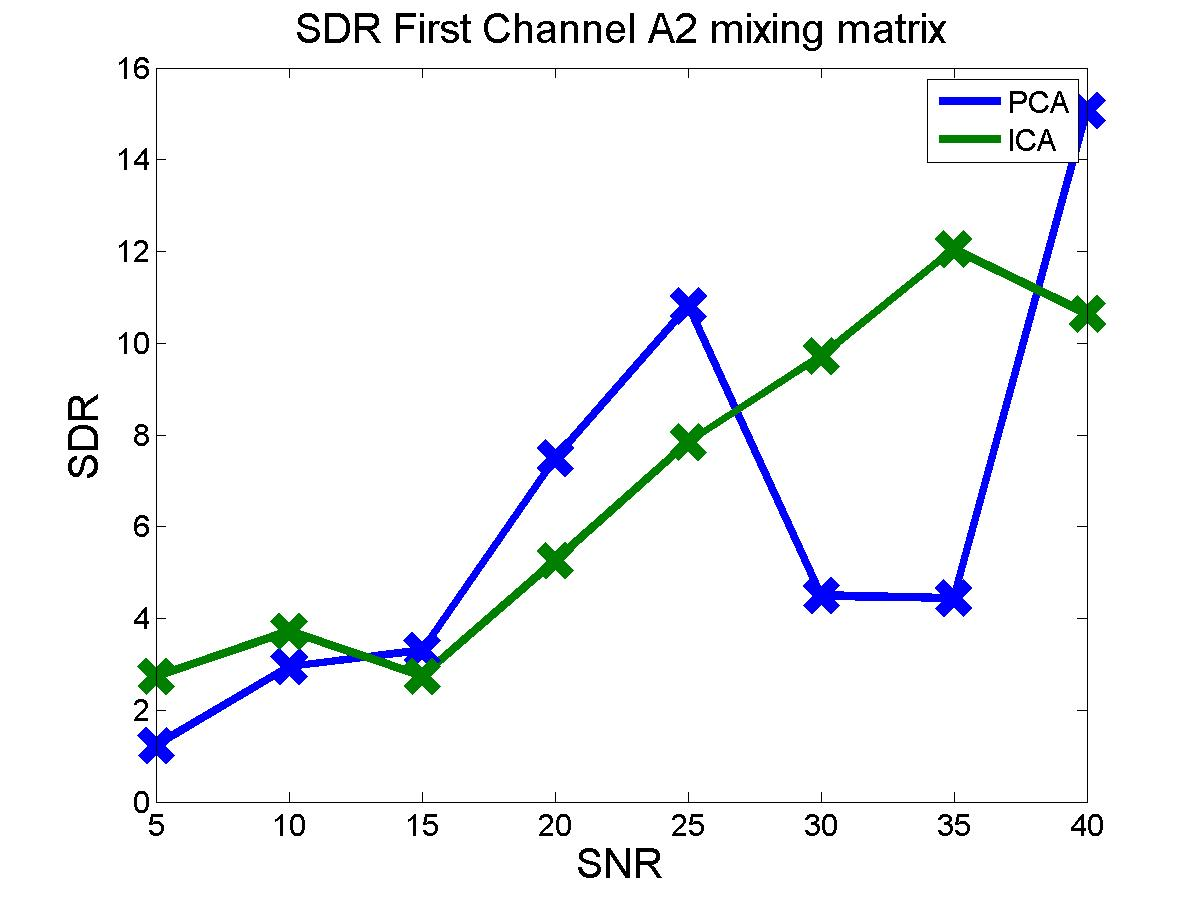
\includegraphics[width=.6\textwidth]{3.jpg}\\
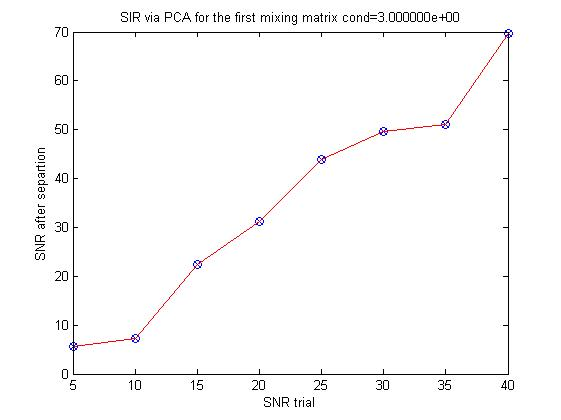
\includegraphics[width=.6\textwidth]{SNR3.jpg}\\
\tiny{First mixing matrix}\label{a3}
\endminipage\hfill
\minipage{.47\textwidth}%
\centering
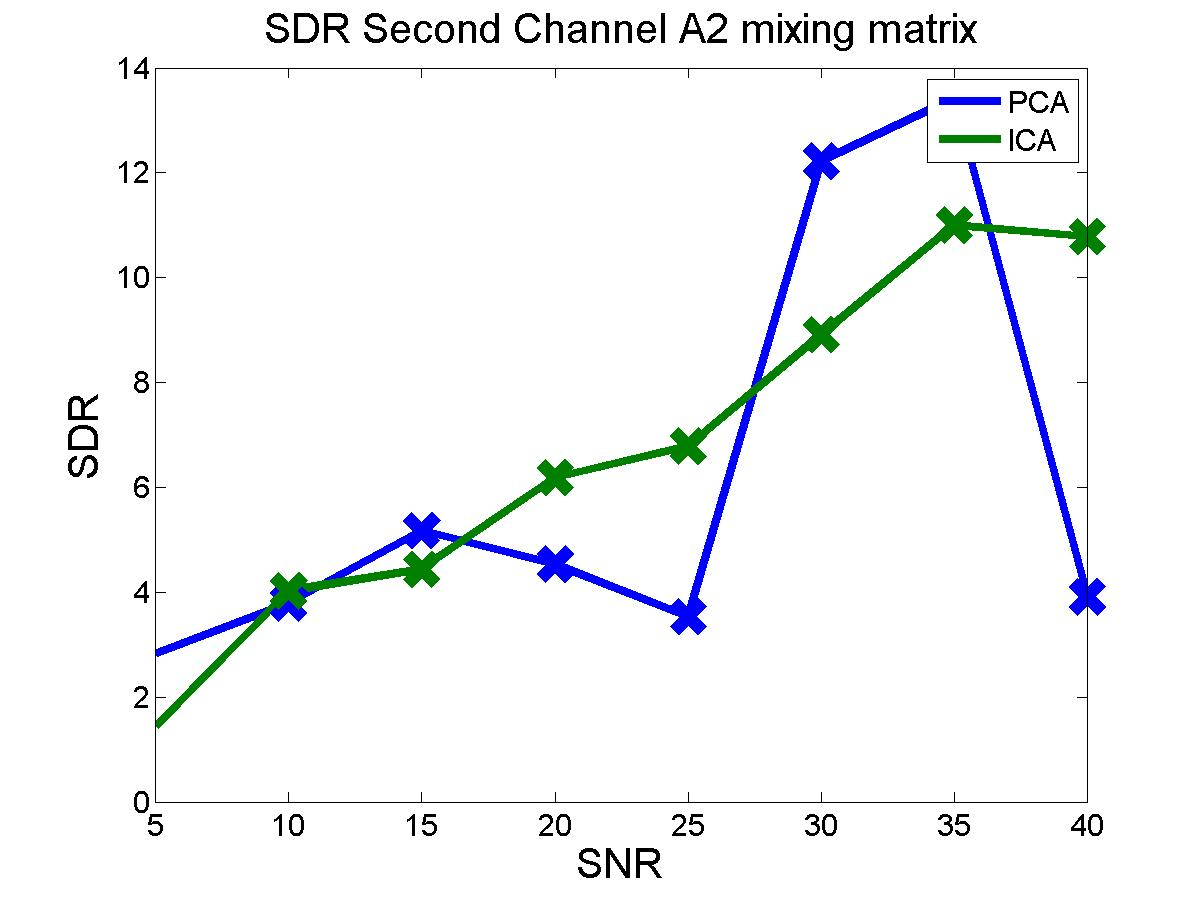
\includegraphics[width=.6\textwidth]{4.jpg}\\
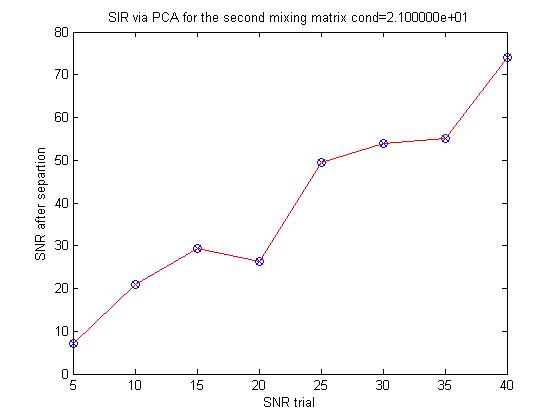
\includegraphics[width=.6\textwidth]{SNR4.jpg}\\
\tiny{Second mixing matrix}\label{a4}
\endminipage\hfill
\caption{\tiny Performance of PCA Implementation}\label{a2}
\end{figure}


\begin{figure}[!htbp]
\minipage{.47\textwidth}%
\centering
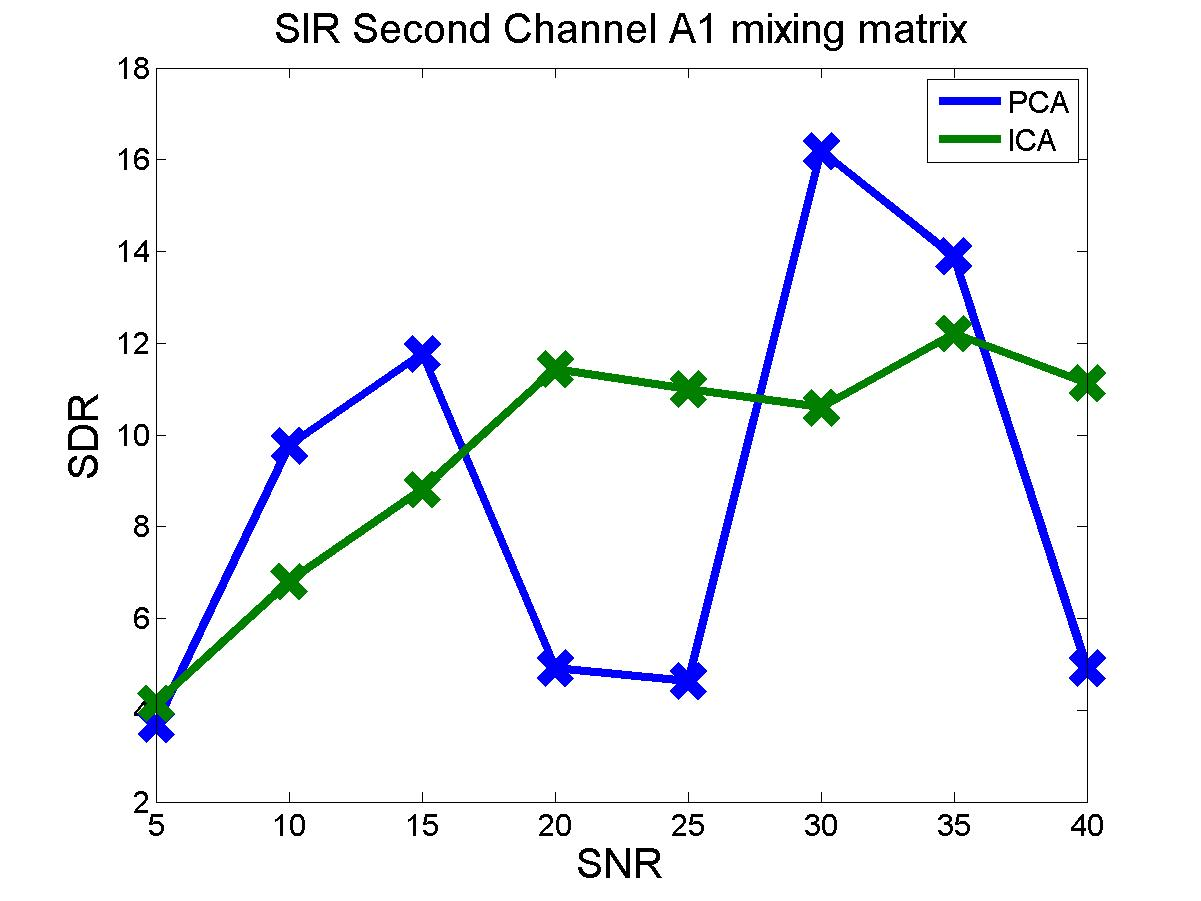
\includegraphics[width=1\textwidth]{6.jpg}
\subcaption{Channel data before ICA}\label{a9}
\endminipage\hfill
\minipage{.47\textwidth}%
\centering
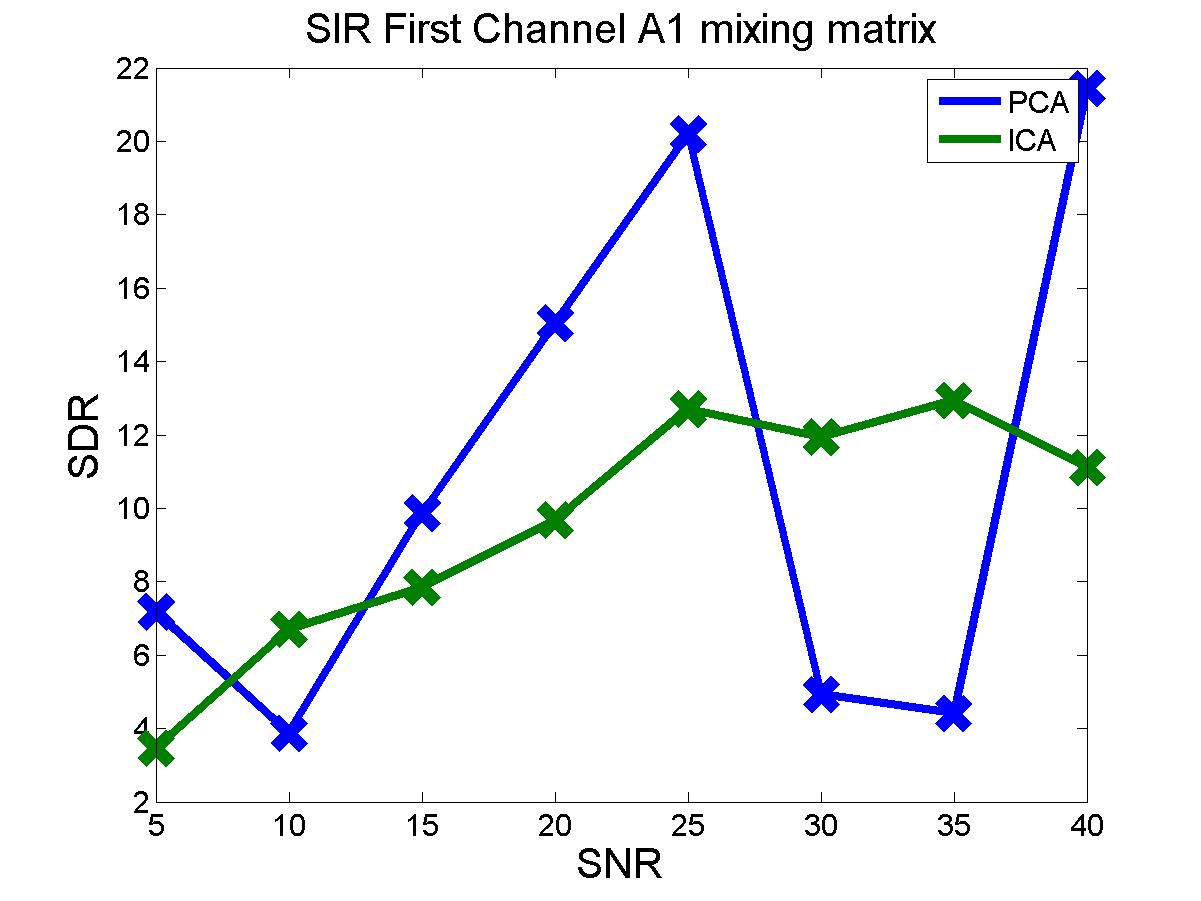
\includegraphics[width=1\textwidth]{5.jpg}
\subcaption{Channel after before ICA}\label{a10}
\endminipage\hfill
\caption{ICA separation via COM2 method}
\end{figure}



\begin{figure}[!htbp]
\minipage{.3\textwidth}%
\centering
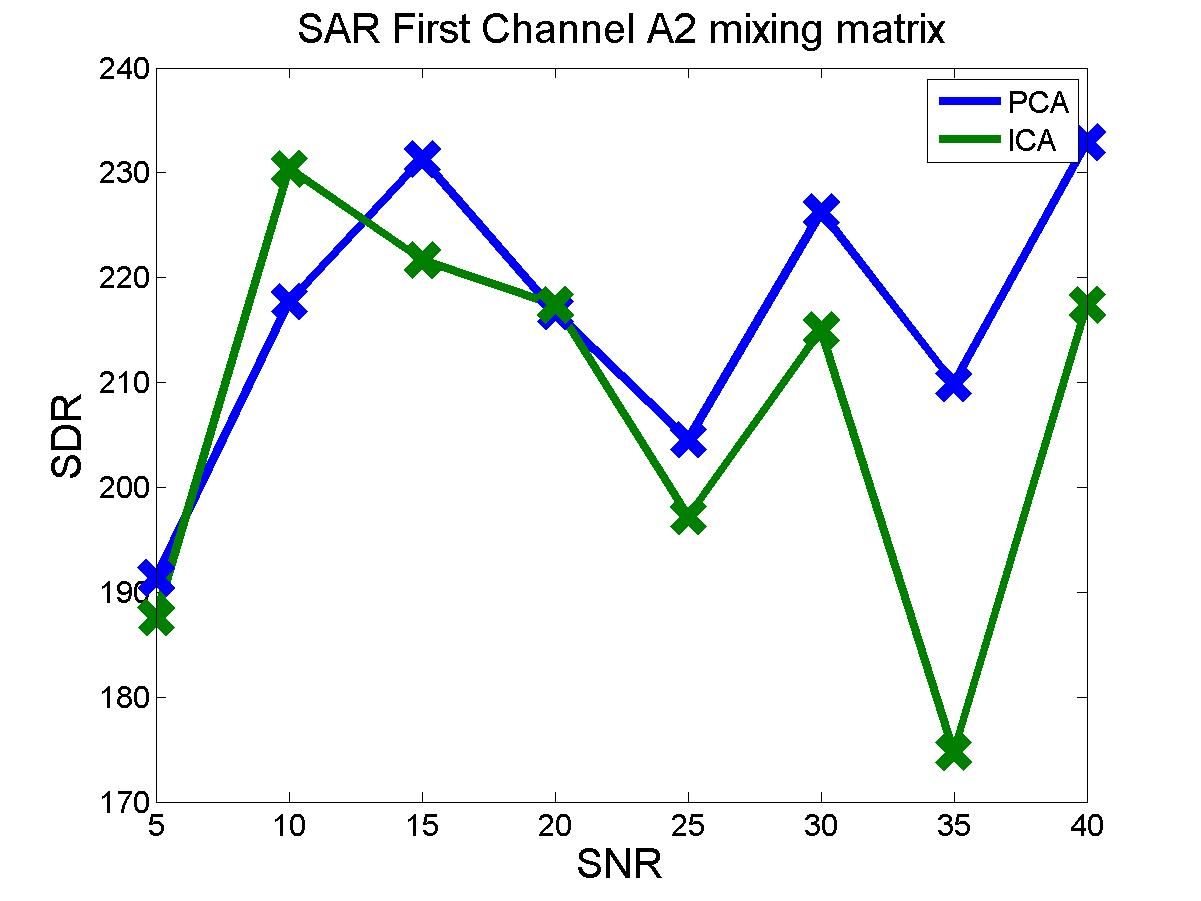
\includegraphics[width=1\textwidth]{11.jpg}
\endminipage\hfill
\minipage{.3\textwidth}%
\centering
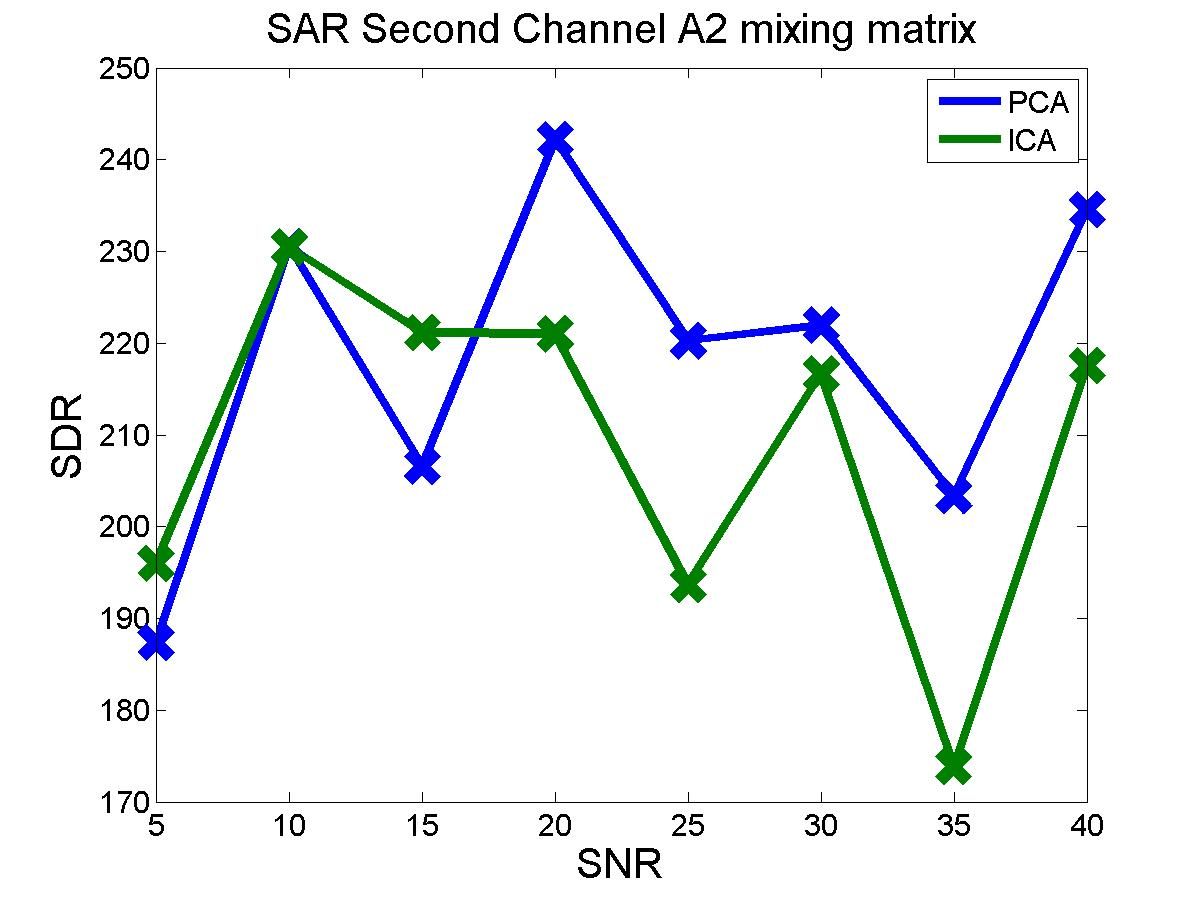
\includegraphics[width=1\textwidth]{12.jpg}
\endminipage\hfill
\minipage{.3\textwidth}%
\centering
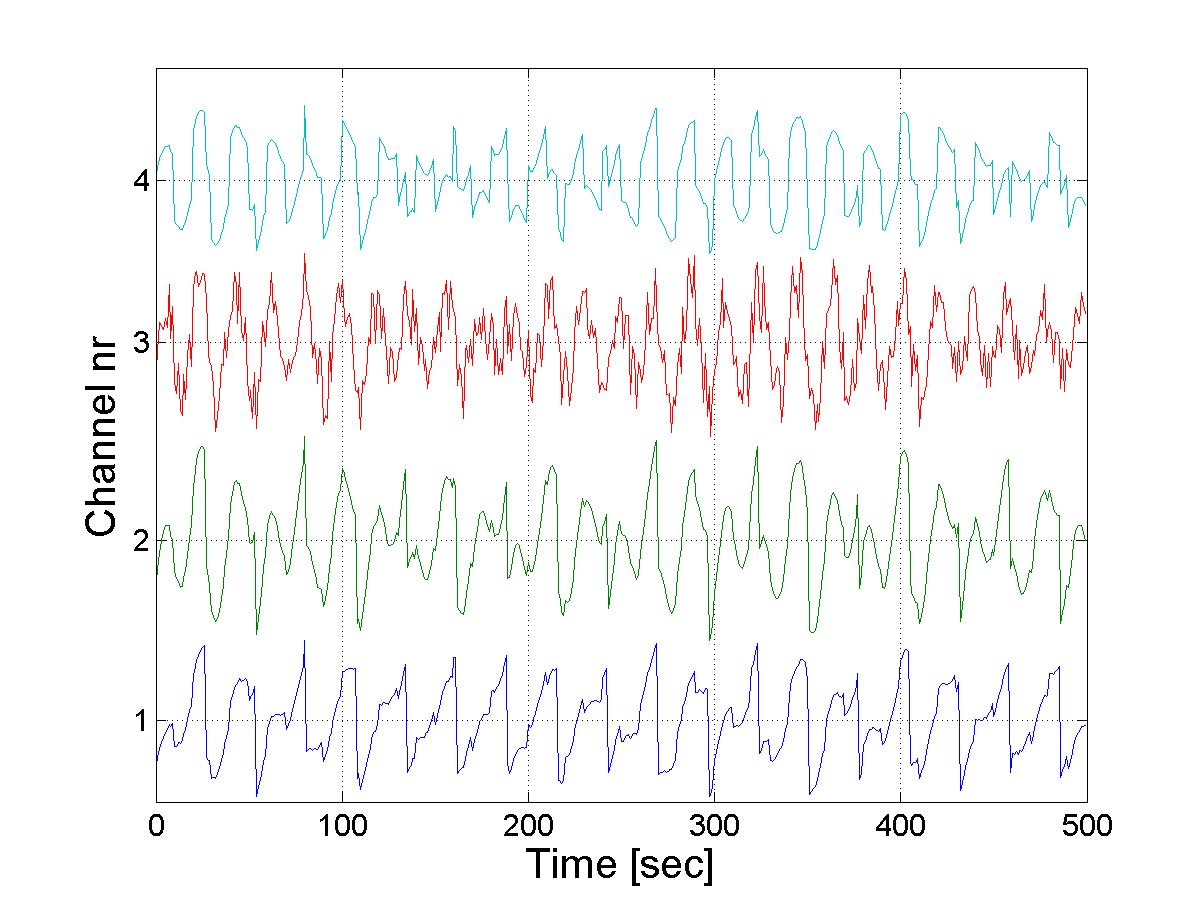
\includegraphics[width=1\textwidth]{13.jpg}
\endminipage\hfill
\caption{CPD components}\label{a15}
\end{figure}

\begin{figure}[!htbp]
\minipage{.3\textwidth}%
\centering
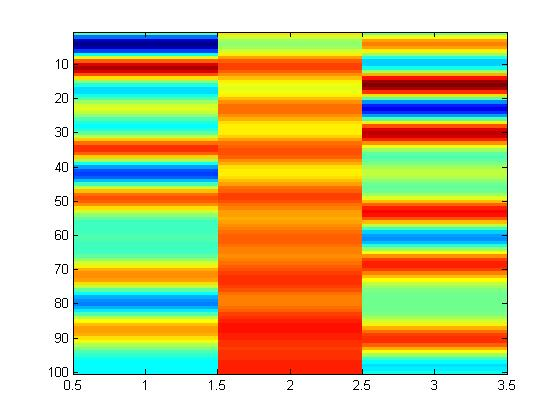
\includegraphics[width=1\textwidth]{26.jpg}
\endminipage\hfill
\minipage{.3\textwidth}%
\centering
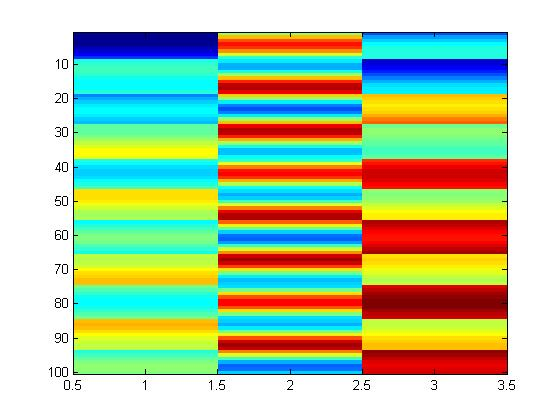
\includegraphics[width=1\textwidth]{25.jpg}
\endminipage\hfill
\minipage{.3\textwidth}%
\centering
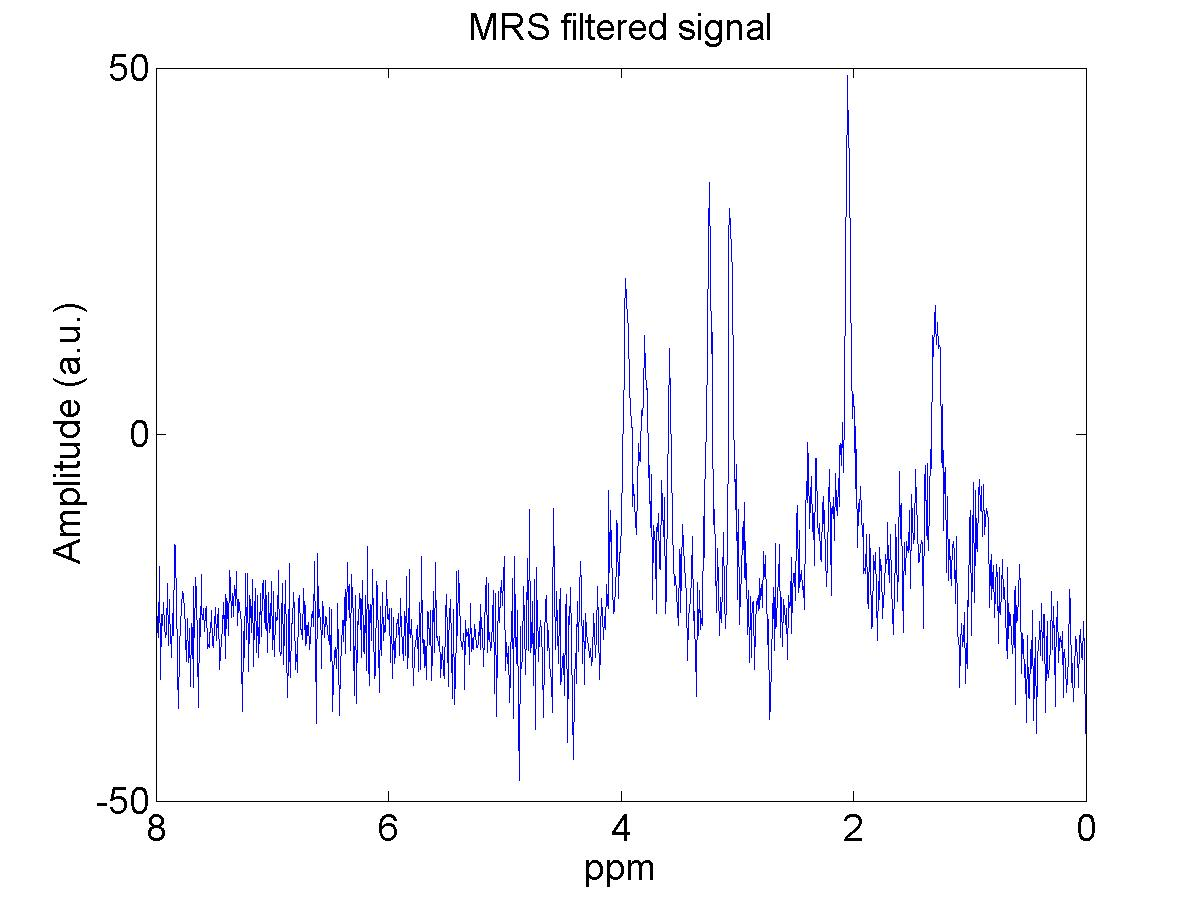
\includegraphics[width=1\textwidth]{24.jpg}
\endminipage\hfill
\caption{Components via SVD}\label{A1}
\end{figure}


\begin{figure}[!htbp]
\minipage{.47\textwidth}%
\centering
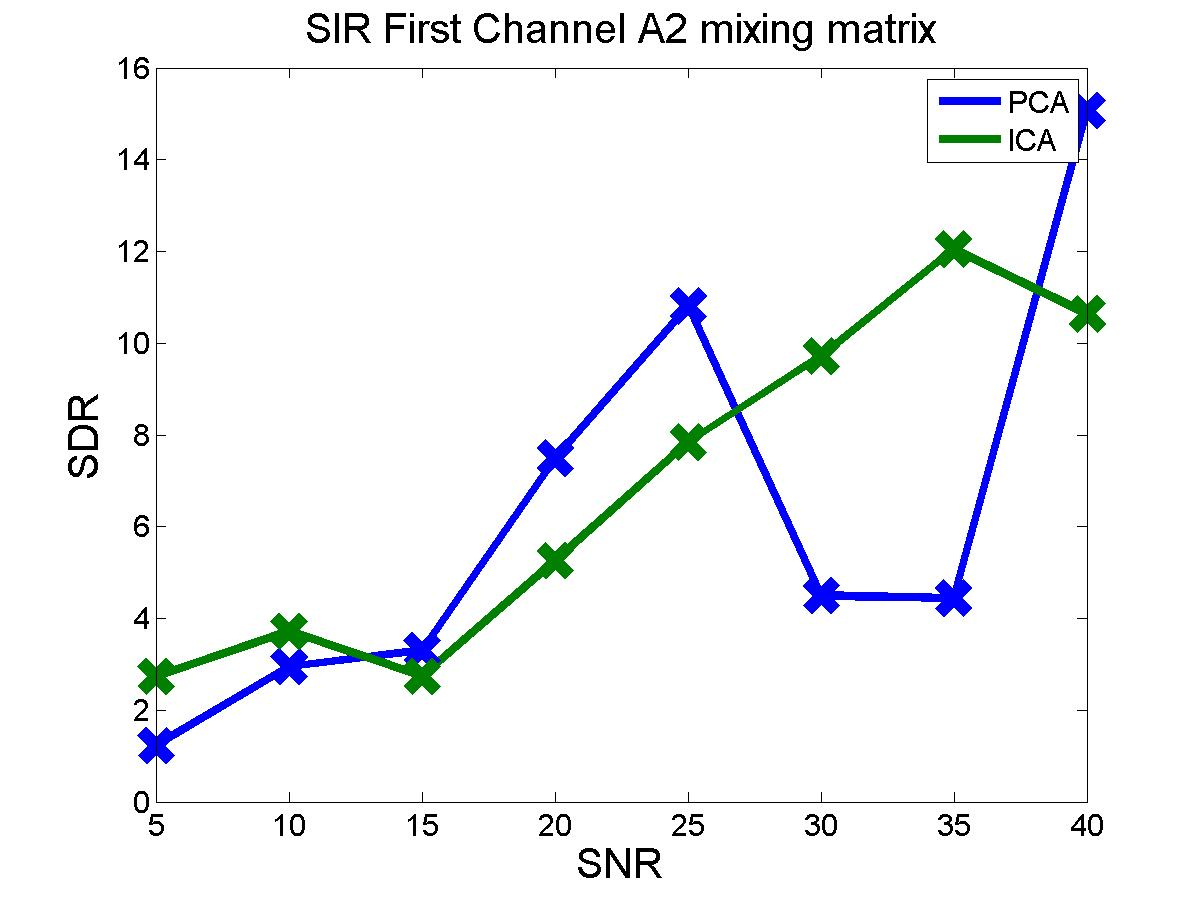
\includegraphics[width=1\textwidth]{7.jpg}
\subcaption{Freb norm over different iteration}\label{a13}
\endminipage\hfill
\minipage{.47\textwidth}%
\centering
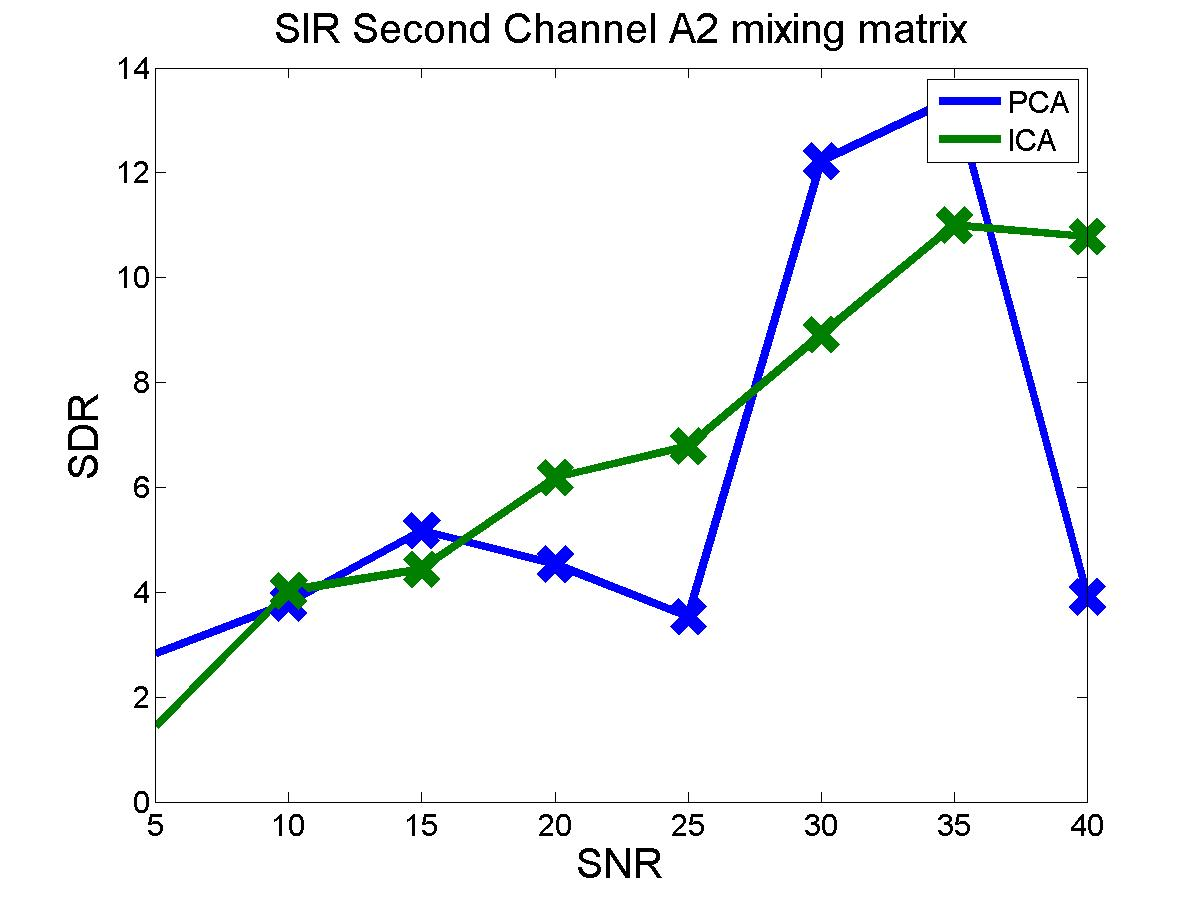
\includegraphics[width=1\textwidth]{8.jpg}
\subcaption{Relative error of estiamtion}\label{a14}
\endminipage\hfill
\caption{CPD estimation}
\end{figure}




\begin{figure}[!htbp]
\minipage{.47\textwidth}%
\centering
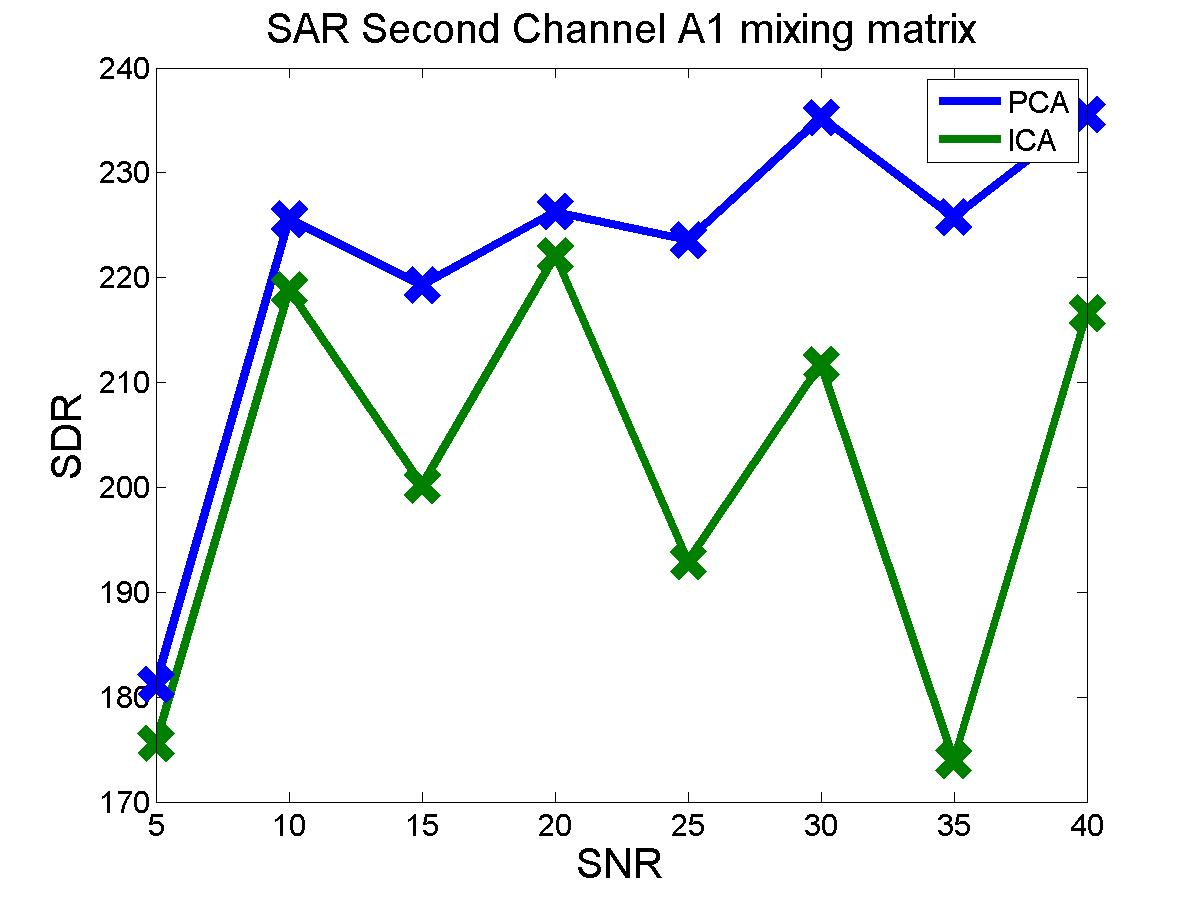
\includegraphics[width=1\textwidth]{10.jpg}
\subcaption{Multilinear singular values in the noisy case}\label{a11}
\endminipage\hfill
\minipage{.47\textwidth}%
\centering
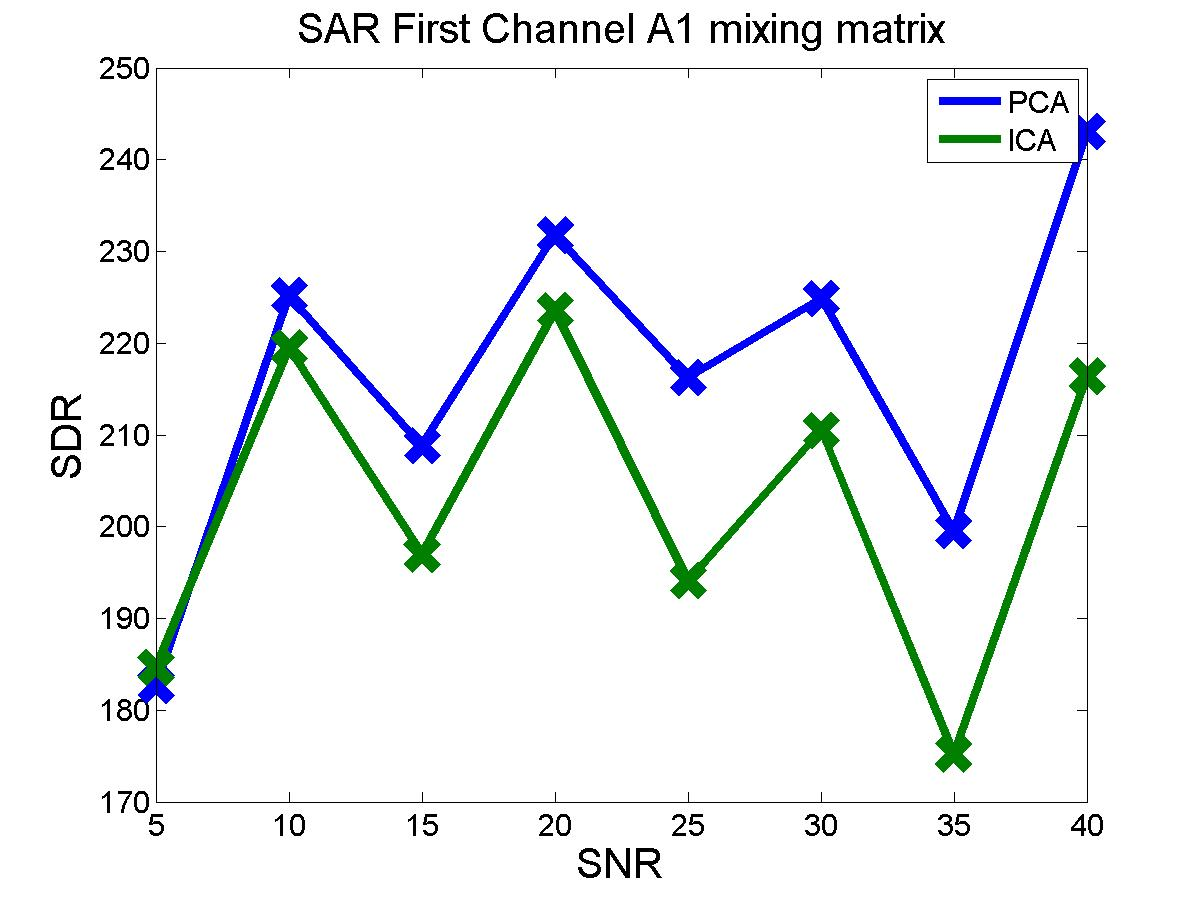
\includegraphics[width=1\textwidth]{9.jpg}
\subcaption{Multilinear singular values in the noiseless case}\label{a12}
\endminipage\hfill
\caption{CPD}
\end{figure}

\begin{figure}[!htbp]
\minipage{.3\textwidth}%
\centering
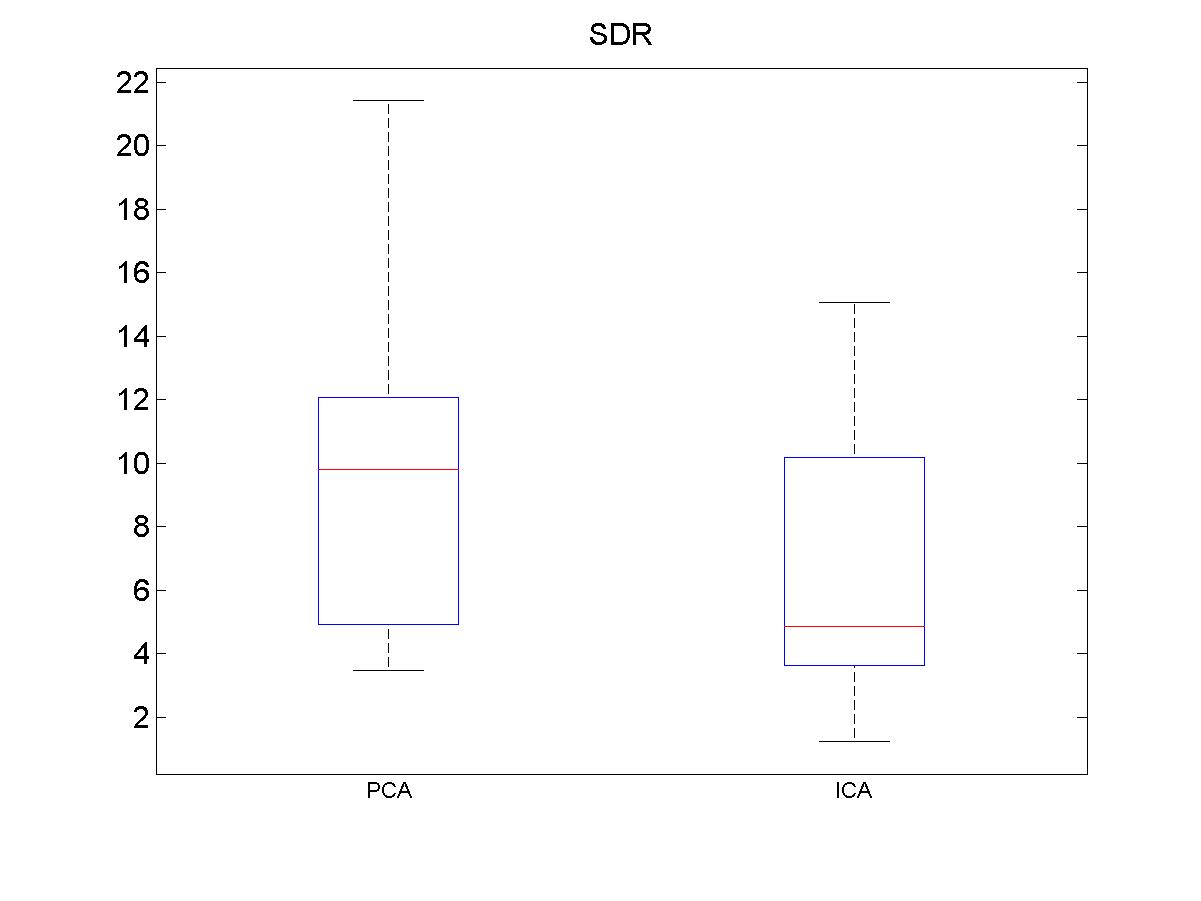
\includegraphics[width=1\textwidth]{15.jpg}
\endminipage\hfill
\minipage{.3\textwidth}%
\centering
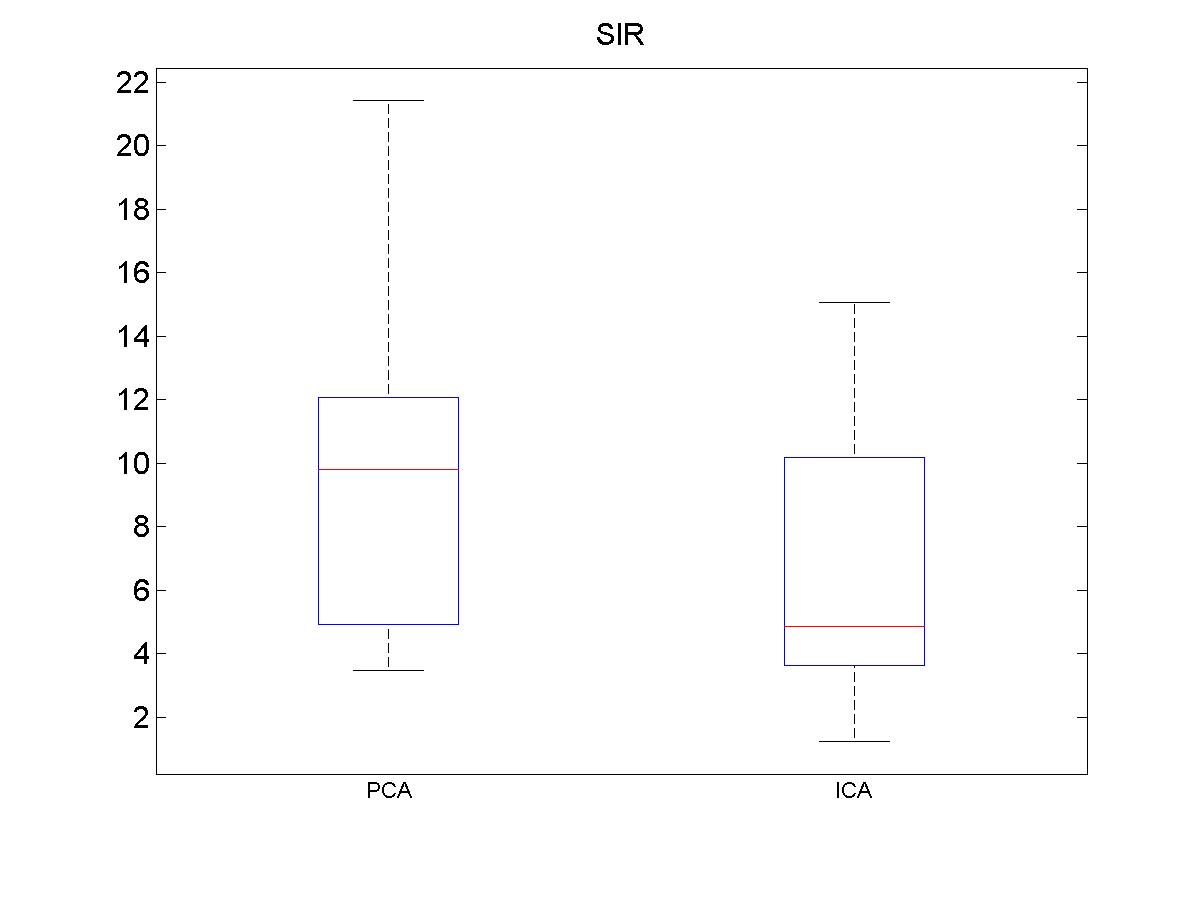
\includegraphics[width=1\textwidth]{16.jpg}
\endminipage\hfill
\minipage{.3\textwidth}%
\centering
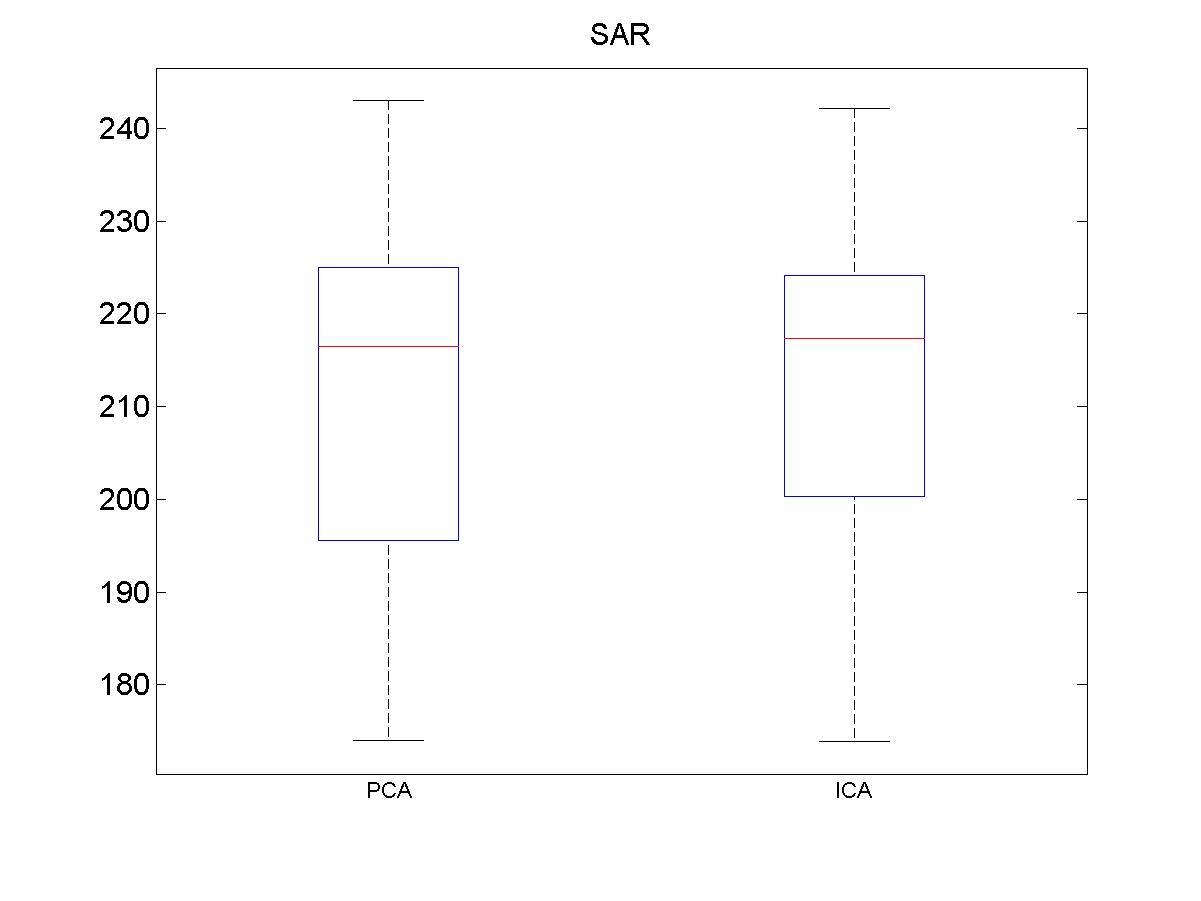
\includegraphics[width=1\textwidth]{17.jpg}
\endminipage\hfill
\caption{Tensorization of the EEG signals}\label{a16}
\end{figure}

\begin{figure}[!htbp]
\centering
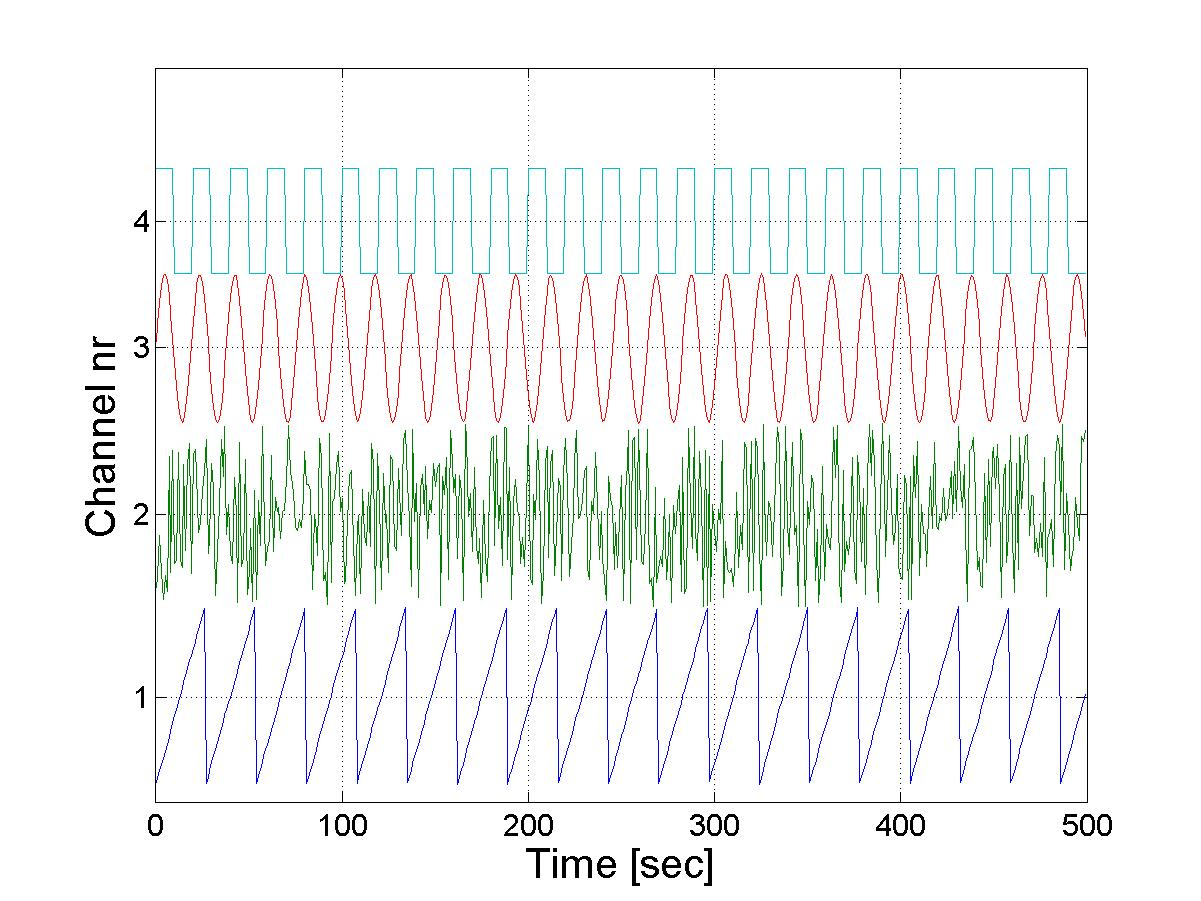
\includegraphics[width=.6\textwidth]{14.jpg}
\caption{Channel data}\label{a17}

\end{figure}


\begin{figure}[!htbp]
\minipage{.47\textwidth}%
\centering
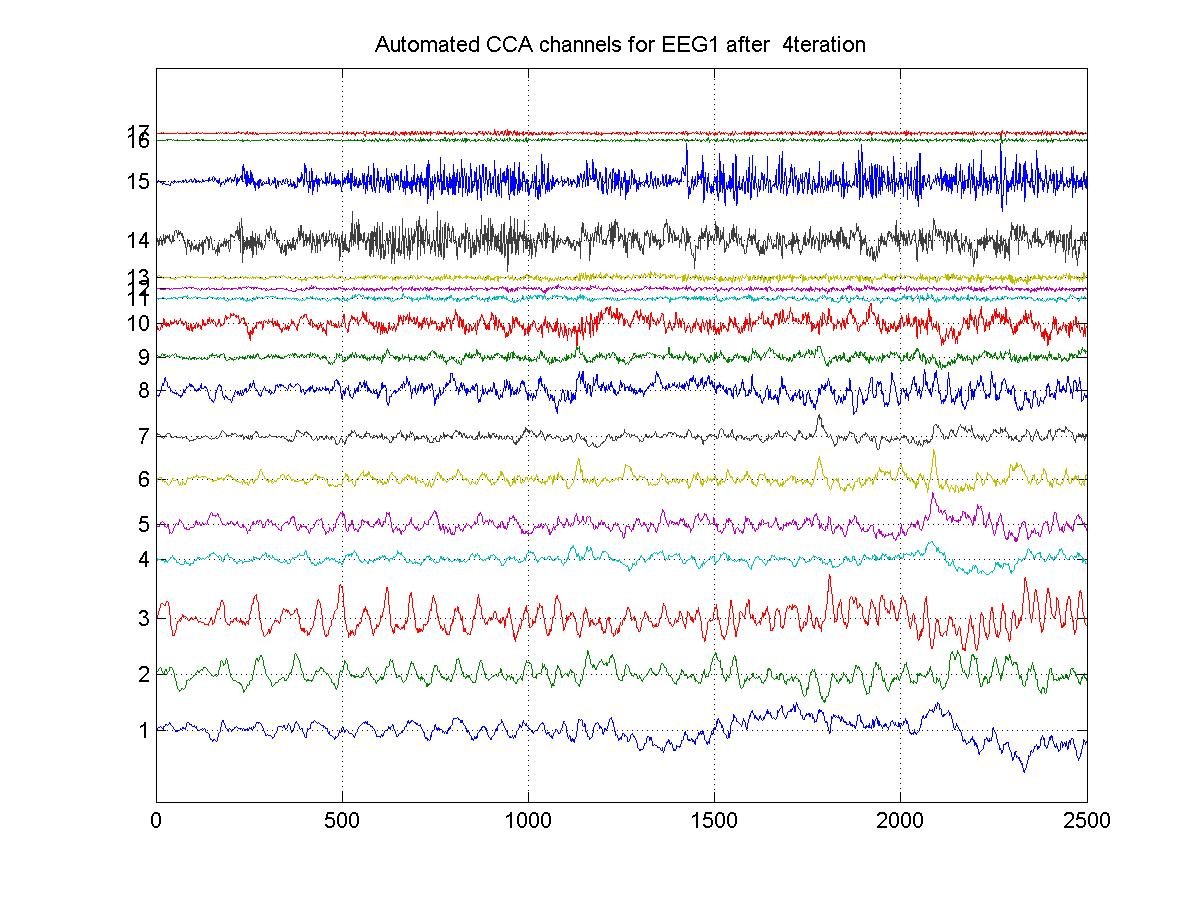
\includegraphics[width=1\textwidth]{18.jpg}
\subcaption{Time resoltution}\label{a18}
\endminipage\hfill
\minipage{.47\textwidth}%
\centering
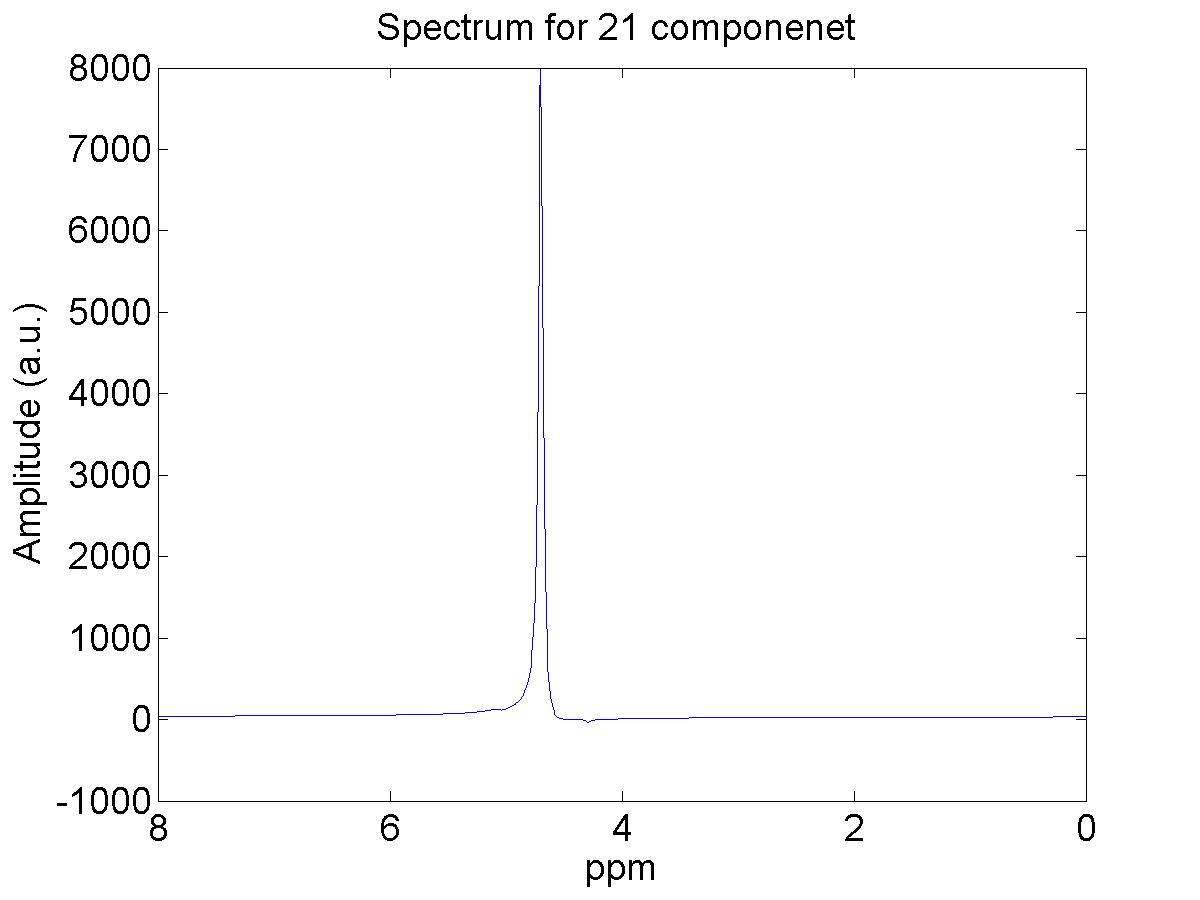
\includegraphics[width=1\textwidth]{19.jpg}
\subcaption{Frequency resolution}\label{a19}
\endminipage\hfill
\caption{Multilinear singular values}
\end{figure}

\begin{figure}[!htbp]
\minipage{.47\textwidth}%
\centering
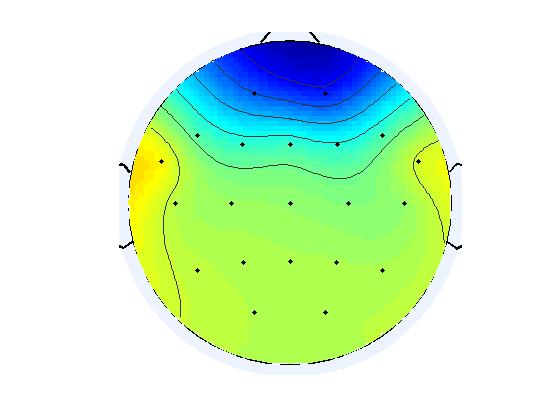
\includegraphics[width=1\textwidth]{20.jpg}
\subcaption{First event}\label{a20}
\endminipage\hfill
\minipage{.47\textwidth}%
\centering
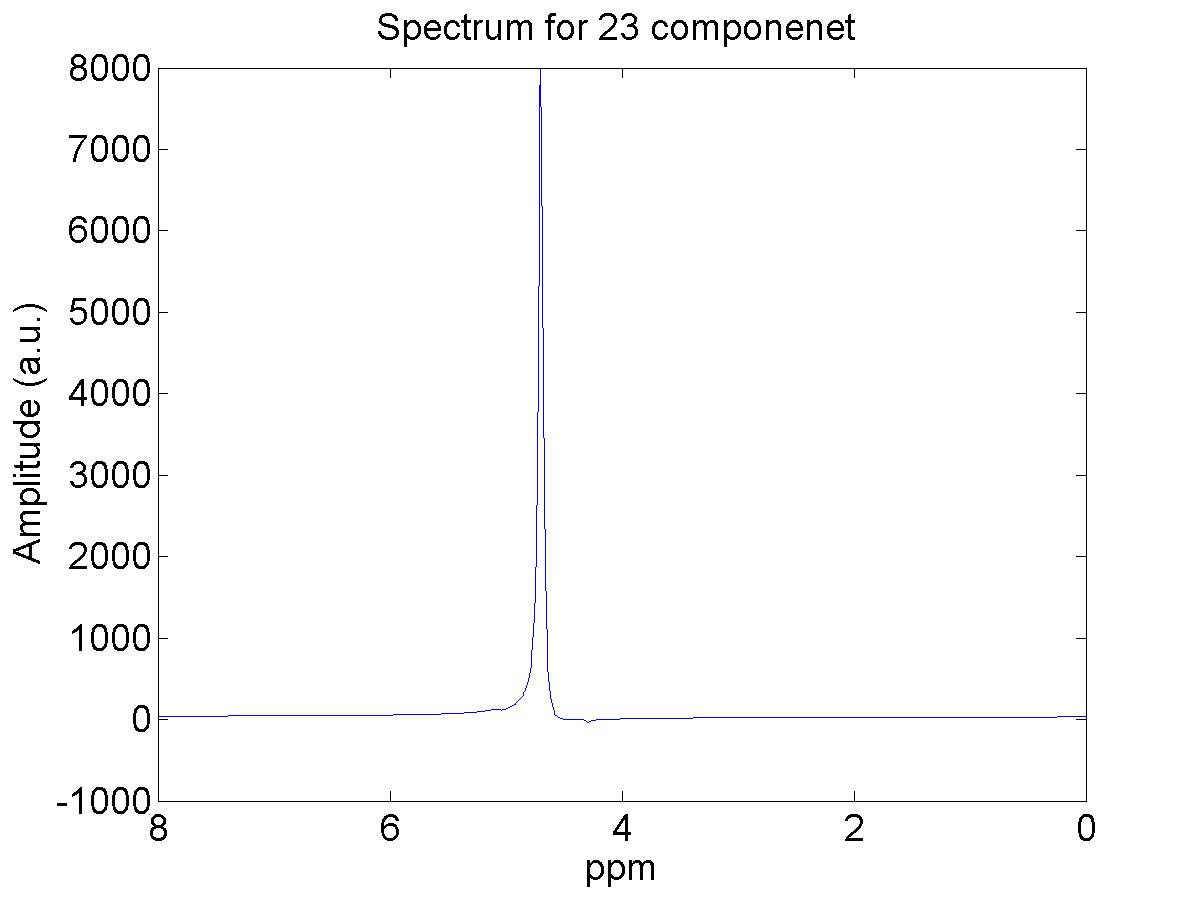
\includegraphics[width=1\textwidth]{21.jpg}
\subcaption{Second event Epilepsy}\label{a21}
\endminipage\hfill
\minipage{.47\textwidth}%
\centering
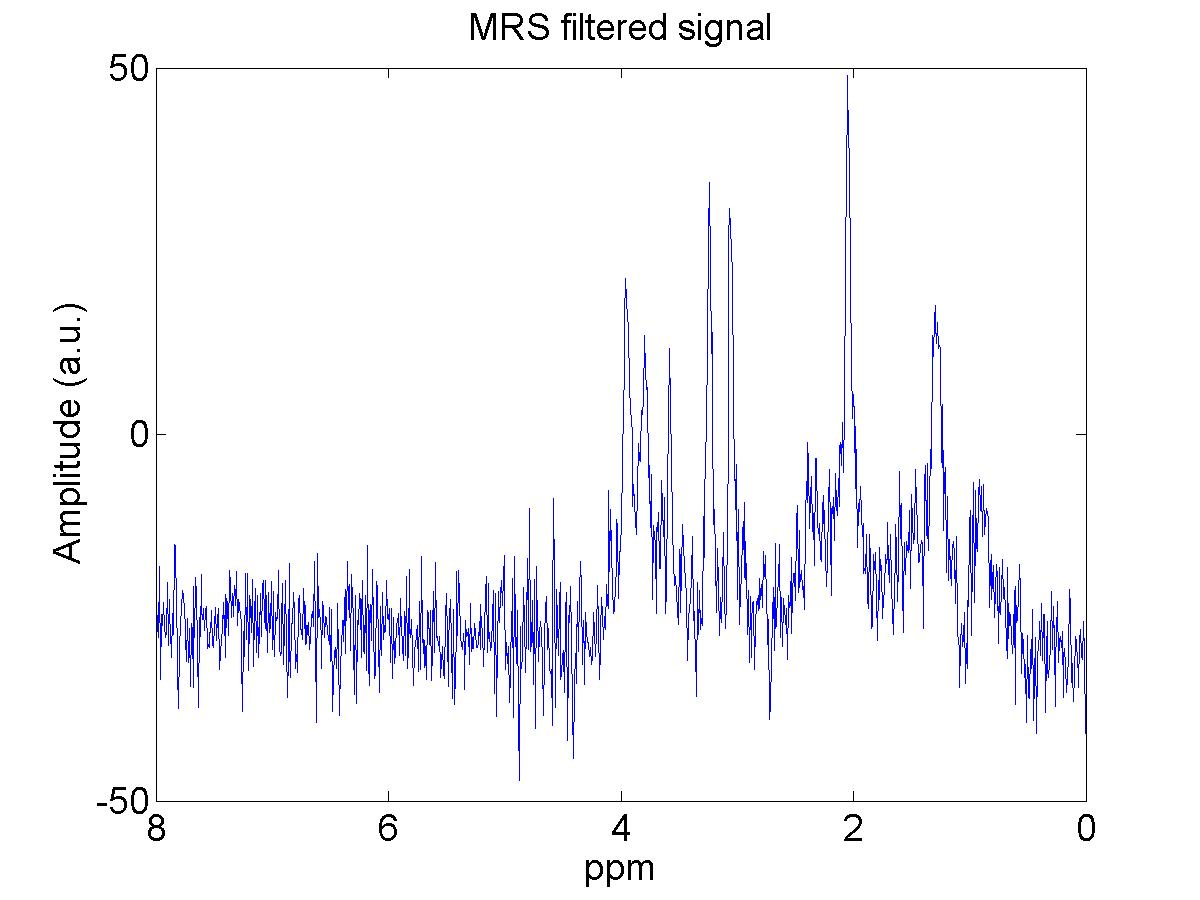
\includegraphics[width=1\textwidth]{22.jpg}
\subcaption{Second event Epilepsy}\label{a22}
\endminipage\hfill
\minipage{.47\textwidth}%
\centering
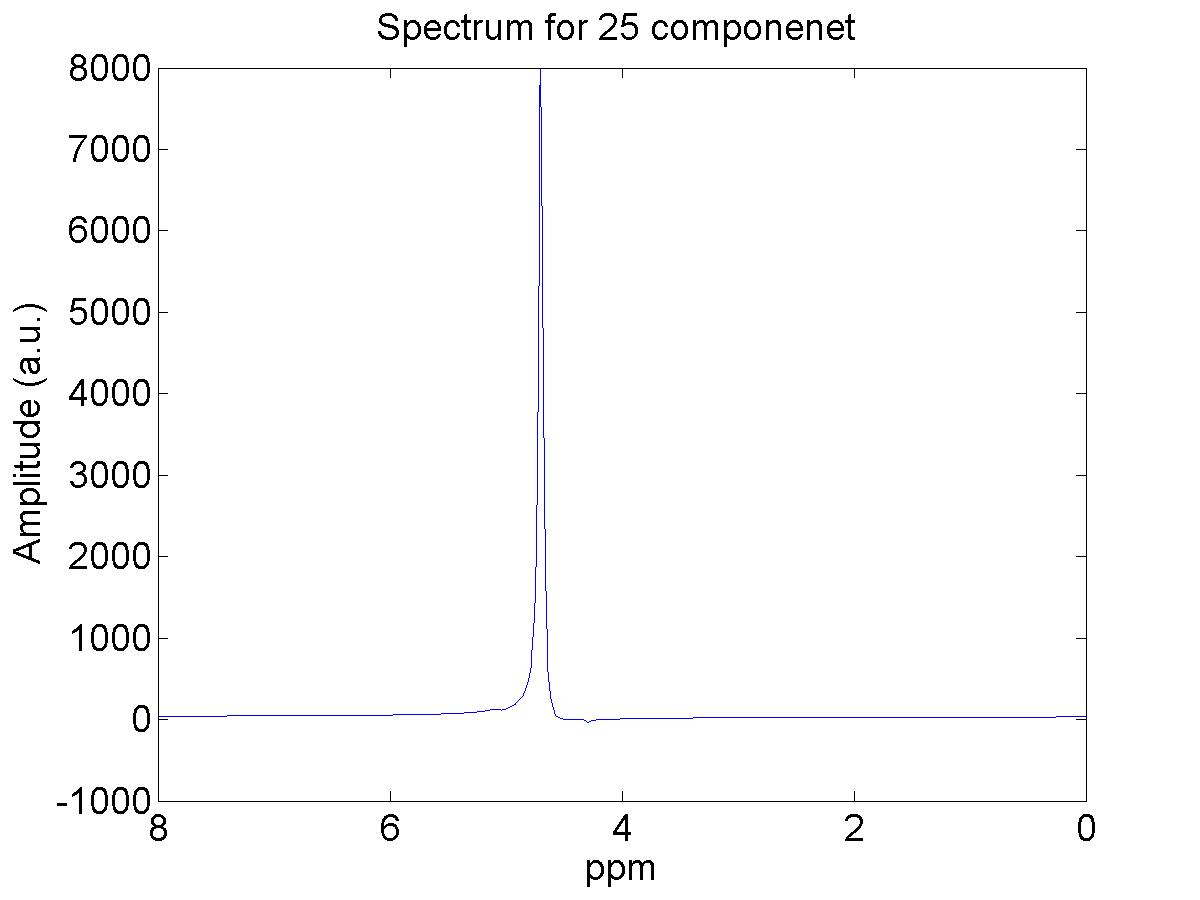
\includegraphics[width=1\textwidth]{23.jpg}
\subcaption{Second event Epilepsy}\label{a23}
\endminipage\hfill
\caption{Voltage profile for the normal brain activity in a) and Epilepsy in the rest of the maps}\label{a}
\end{figure}


\begin{figure}[!htbp]
\centering
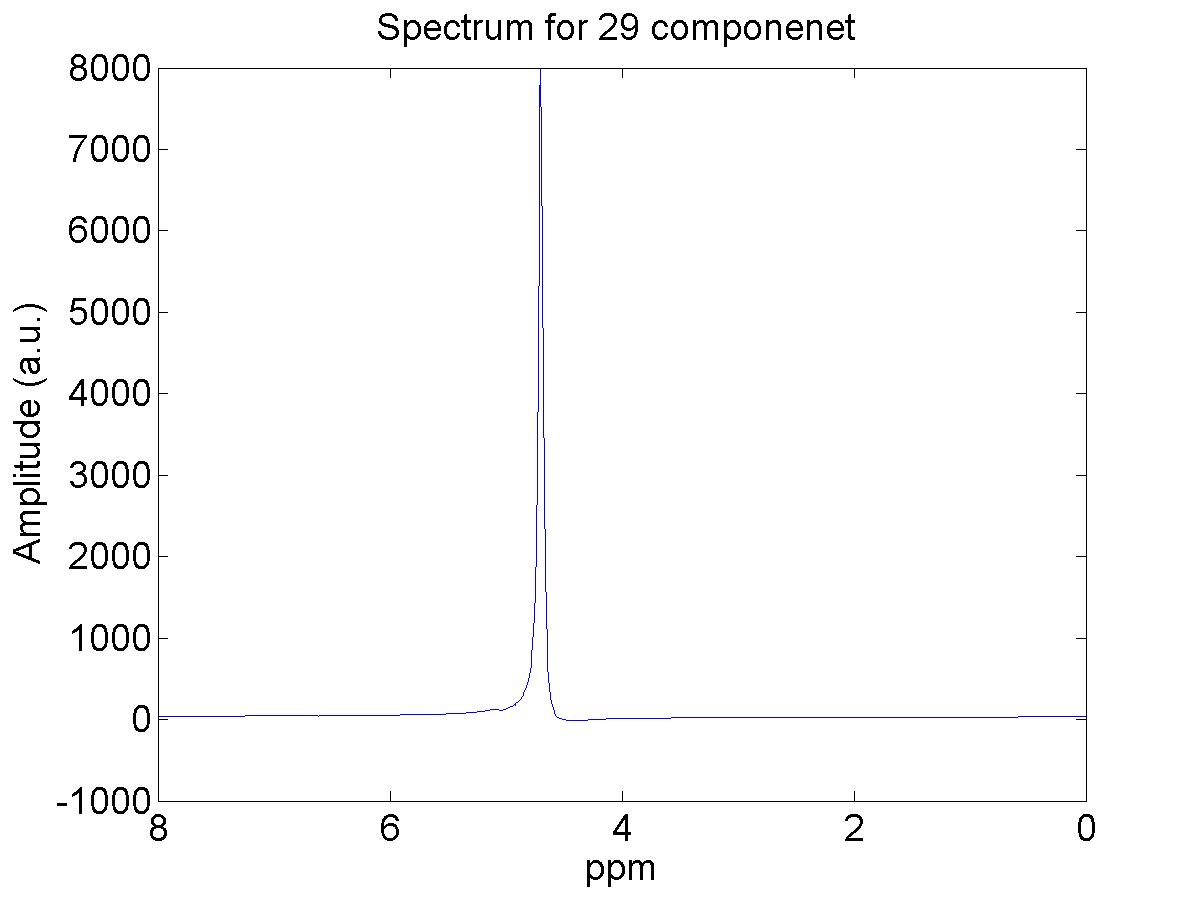
\includegraphics[width=.6\textwidth]{27.jpg}
\caption{Rank estimation}\label{A2}

\end{figure}



\bibliographystyle{unsrt}
\bibliography{Bibliography}

\clearpage
\appendix

\section{Additional figure}


\lstset{language=Matlab,%
    %basicstyle=\color{red},
    breaklines=true,%
    morekeywords={matlab2tikz},
    keywordstyle=\color{blue},%
    morekeywords=[2]{1}, keywordstyle=[2]{\color{black}},
    identifierstyle=\color{black},%
    stringstyle=\color{mylilas},
    commentstyle=\color{mygreen},%
    showstringspaces=false,%without this there will be a symbol in the places where there is a space
    numbers=left,%
    numberstyle={\tiny \color{black}},% size of the numbers
    numbersep=9pt, % this defines how far the numbers are from the text
    emph=[1]{for,end,break},emphstyle=[1]\color{red}, %some words to emphasise
    %emph=[2]{word1,word2}, emphstyle=[2]{style},    
}




\newpage
\subsection{Source Code}
\lstinputlisting{MainExceriseSession.m}
\lstinputlisting{PlotEEG.m}
\lstinputlisting{PlotSIR.m}




\end{document}

